\documentclass[a4paper,spanish]{article}

\usepackage{url}
\usepackage{tabu}
\usepackage{float}
\usepackage{cite}
\usepackage[spanish]{cleveref}
\usepackage[colorlinks]{hyperref}
\usepackage{fancyvrb}

\bibliographystyle{unsrt}

\usepackage[activeacute]{babel}
\usepackage{fancyhdr}
\usepackage{ecarat}
\usepackage{graphicx}
%\usepackage{amssymb}
\usepackage{amssymb,amsmath}
%\usepackage[all]{xy}
\usepackage{graphicx}
\usepackage{listings}
%\usepackage{pseudocode}
\usepackage[utf8]{inputenc}
%\usepackage{wrapfig}
\usepackage{lastpage}
\usepackage{multicol}
\usepackage{url}
\usepackage{color}
\usepackage{array}
\usepackage{url}
\usepackage{listings}
\usepackage{sverb}



\graphicspath{
{./imgs/}
}

\usepackage{xifthen}% provides \isempty test
%~ \usepackage{ulem}%para subrayados
\usepackage{dashrule}%para subrayados

%~ \usepackage{relacion}

\oddsidemargin 0in
\textwidth 6.5in
\topmargin 0in
\addtolength{\topmargin}{-.4in}
\addtolength{\leftmargin}{-.5in}
\textheight 10in
\parskip=1ex
\pagestyle{fancy}
\newcommand{\real}{\hbox{\bf R}}
\newcommand{\prima}{^{\prime}}
\newcommand{\tab}{\hspace*{1cm}}
%Cosas que se usan en el enunciado
% \parindent = 0 pt
% \parskip = 11 pt

\usepackage{a4wide}
\newcommand{\erf}{\hbox{erf}}
\newcommand\abs[1]{\ensuremath{\left| {#1} \right|}}
%~ \addtolength{\textheight}{1cm}

\lstdefinelanguage{Smalltalk}{ 
	morekeywords={true,false,self,super,nil}, 
	sensitive=true, 
	morecomment=[s]{"}{"}, 
	morestring=[d]', 
	style=SmalltalkStyle 
} 
\lstdefinestyle{SmalltalkStyle}{ 
	literate={:=}{{$\gets$}}1{^}{{$\uparrow$}}1 
} 
\lstset {%
     language=Smalltalk,
     frame=l,
     framerule=1pt,
     aboveskip=1em,
     framextopmargin=3pt,
     framexbottommargin=3pt,
     framexleftmargin=0.4cm,
     framesep=0pt,
     rulesep=.4pt,
     %~ backgroundcolor=\color{gris95},
     rulesepcolor=\color{red},
     tabsize=4,
     %
     stringstyle=\sffamily,
     showstringspaces = false,
     basicstyle=\footnotesize\sffamily,
     identifierstyle=,
     commentstyle=\em, %\sffamily\color{gris50},
     keywordstyle=\bfseries,
     commentstyle=\scriptsize\sffamily,
     breaklines=true,
     breakatwhitespace=true,
     morekeywords={setof},
   }

\usepackage{longtable}




\begin{document}

\materia{Metaheurísticas}
\submateria{Segundo Cuatrimestre de 2015}
\titulo{Trabajo Práctico Final}
\subtitulo{Sudoku }
\abst{}
\grupo{}
\claves{}
\integrante{Emiliano Mancuso}{597/07}{emiliano.mancuso@gmail.com}
\integrante{Gloria Diodati}{285/05}{gloriadiodati@gmail.com}
\integrante{Emiliano Hoss}{664/04}{emihoss@gmail.com}



\cfoot{$\thepage$ de \pageref{LastPage}}

\thispagestyle{empty}

\maketitle



\tableofcontents
\pagebreak


\section{Resumen}
En el siguiente trabajo práctico resolveremos un problema NP-Completo llamado
Sudoku. Mostraremos una estrategia de resolución exacta y una metaheurística
para resolver el problema. Finalmente mostraremos los resultados de aplicar la
metaheurística.


\section{Introducción}
\label{sec:intro}

El juego \emph{Sudoku} es un rompecabezas lógico que trata la ubicación de
números en una grilla de $N^2 x N^2$. Este tiene celdas con valores ya fijados,
llamados \textit{pistas}, y el objetivo es completar las celdas
faltantes con valores de $1..N^2$. La grilla se subdivide en $N$ cuadrantes de
$N x N$  y se debe completar cumpliendo con las siguientes reglas:

\begin{enumerate}
    \label{enum:principios}

    \item Cada fila debe tener los valores de 1 a N una única vez
    \item Cada columna debe tener los valores de 1 a N una única vez
    \item Cada subcuadrante de $NxN$ debe tener los valores de 1 a N una única vez
\end{enumerate}

Un ejemplo de este tipo de problemas tan conocido se observa en la tabla
\ref{img:sudoku}


\begin{figure}[H]
	\centering
	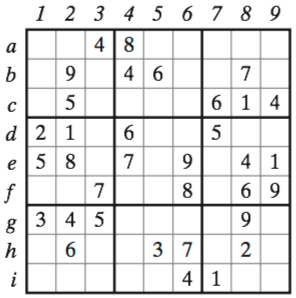
\includegraphics[scale=0.6]{./img/sudoku.png}
	\caption{Sudoku ejemplo}
	\label{img:sudoku}
\end{figure}

Durante los últimos tiempos, han surgido diversos métodos para resolver
de manera heurística el problema dada su complejidad.

Los métodos de resolución exacta para este problema con \emph{Fuerza bruta}
consisten en asignar posibles valores iterativamente a las celdas e ir
verificando si el sudoku cumple las reglas a medida que se siguen completando
los blancos.

Este algoritmo de resolución es costoso y a menudo se utiliza con backtracking.


En la actualidad se han encontrado avances en la resolución de Sudoku utilizando
algoritmos genéticos \cite{mantere}, Búsqueda armónica
\cite{harmony} y Ant Colony \cite{ant_colony} entre otros.

Para este trabajo práctico, implementamos una metaheurística de Ant Colony, y una
de búsqueda local, que transforma el Sudoku en un problema de coloreo de grafos y
luego utiliza DSatur\cite{dsatur} como heurística.


\section{Búsqueda Local - DSatur}

Supongamos que tenemos un problema al que queremos encontrarle una solución
óptima, este problema toma diversos parámetros y por cada instancia
devuelve una solución que puede ser correcta en términos de las restricciones
del problema, puede ser óptima en términos de ser la mejor solución, o puede ser
ninguna de las anteriores. En este último caso, evaluaremos si siguiendo por esa
solución parcial del problema alcanzaremos una solución que sea a la vez
correcta y óptima.

Una solución óptima puede no ser siempre alcanzable y en ese caso se busca la
mejor solución. Se dice que una solución $S_1$ es mejor que solución $S_2$ si
dada una función objetivo  que toma instancias de solución nos permite
compararlas para determinar si una es mejor que la otra.

\begin{equation}
    f(S_1) < f(S_2) 
\end{equation}


El método de Búsqueda local entonces, itera sobre el espacio de soluciones
buscando en cada paso obtener una mejor solución parcial hasta alcanzar un
mínimo. Luego de la estabilización, este se detiene.

¿Qué sucede si el método no alcanzó el mínimo absoluto? Este se estanca
en una solución que no se encuentra cercana al valor óptimo y terminará
arrojando un mínimo local.


Ahora necesitamos definir como transformamos el problema de resolver un Sudoku
a un problema de coloreo de grafos.
Ademas, definiremos la función objetivo, la función de vecindad y los parámetros.
Para todos los casos, utilizamos los Sudoku de $ 9x9 $.

\subsection{Transformación}
\label{sec:transformacion}

La transformación es bastante trivial, cada celda del Sudoku es representada por
un nodo en el Grafo, y la fila, columna y el subcuadrante asociado son los nodos
adyacentes como muestra \ref{img:adyacentes}.


\begin{figure}[h]
	\centering
	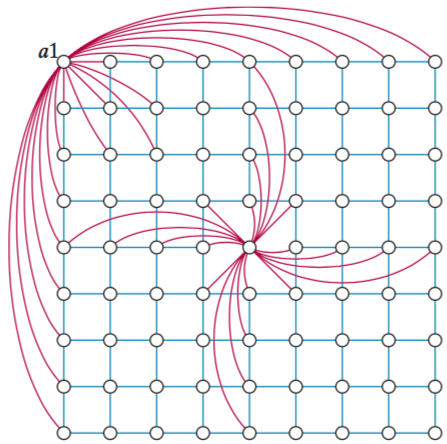
\includegraphics[scale=0.5]{./img/adyacentes.png}
    \caption{Nodos adyacentes}
    \label{img:adyacentes}
\end{figure}

Esta es la estructura básica del grafo, luego tenemos que transformar las pistas
(números que vienen fijos) en colores de manera unívoca. \ref{img:color_map}.

\begin{figure}
	\centering
	
\includegraphics[scale=0.5]{./img/numero_color.png}
    \caption{Asociación de Pistas a Colores}
    \label{img:color_map}
\end{figure}

Con esto, ya contamos con el grafo inicial \ref{img:grafo_inicial} y podemos
comenzar a colorearlo con el algoritmo que elegimos.

\begin{figure}[h]
	\centering
	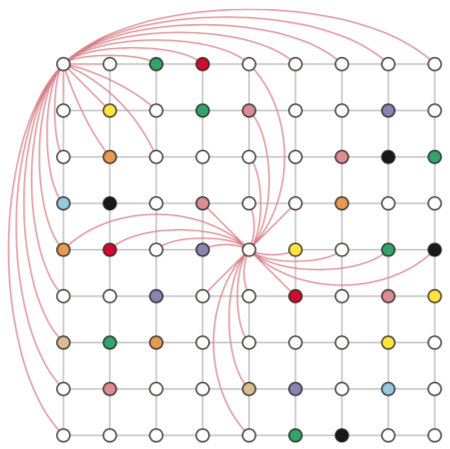
\includegraphics[scale=0.5]{./img/grafo_inicial.png}
    \caption{Grafo Inicial}
    \label{img:grafo_inicial}
\end{figure}

A su vez, de este grafo podemos extraer varias propiedades:

\begin{itemize}
	\item 81 nodos
	\item Clique Máxima: 9
	\item Todo nodo pertenece a una clique máxima
	\item $ grado(n_i) = 20 $
	\item $ \chi(G) = 9 $
\end{itemize}


\subsection{Solución Inicial}

Los algoritmos de coloreo secuencial, también conocidos como coloreo goloso van seleccionando un nodo
de acuerdo a algún criterio específico, formando así un \emph{orden} de coloración.
Luego, en cada nodo lo van coloreando con un color que no tienen sus vecinos.
 
El orden en que se seleccionan los nodos afectan a la coloración, así que un buen orden de
vértices puede traducirse en una buena coloración. No hay ninguna forma de obtener la solución óptima,
sino que, se aplica el algoritmo de coloración secuencial varias veces hasta obtener la coloración válida.

Los algoritmos de colores secuencial proponen las siguiente variantes:

\begin{itemize}
	\item \emph{Largest Degree Ordering (LDO)} - Los vértices son ordenados en orden descendente de acuerdo a su grado. La idea aquí  es que los vértices de mayor grado serán más difíciles de colorear al último, y por eso se colorean primero.
	\item \emph{Saturation Degree Ordering (SDO)} - A diferencia de \emph{LDO} donde el orden de los vértices se determina de antemano, aquí los vértices son seleccionados durante el proceso de coloración. En saturación, el vértice con el grado de saturación más alta se selecciona para ser el próximo a colorear. El grado de saturación de un vértice es el número de colores diferentes usados por sus vecinos. La idea es seleccionar el vértice que está más restringido.
	\item \emph{Incidence Degree Ordering (IDO)} - Es una modificación de \emph{SDO}, el grado de incidencia de un nodo esta definido como el número de vértices adyacentes coloreados.
\end{itemize}
 

\subsection{\emph{SDO}}

Nuestra solución inicial está definida de manera de elegir los nodos con
grado de saturación más alto primero, y asignarles el primer color disponible.

\begin{Verbatim}[samepage=true]
while (ColoredNodes < 81) {
  for all the nodes {
    node = NodeWithMaxSaturatedDegree

    if not colored(node) {
      AssignFirstAvailableColor(node)
      ColoredNodes = ColoredNodes + 1
    }
  }
}
\end{Verbatim}

\subsection{Nodos Conflictivos}

Dado que es un algoritmo goloso, es altamente probable que no de una solución optima.
En los casos que no se pueda asignar un color, o un número del 1-9, el algoritmo
utiliza números mas grandes, y continua buscando una solución.

Decimos que un nodo es conflictivo si cumple la siguiente condición:

\begin{equation}
    hasColor \wedge isNotAClue \wedge ( color > 9 \vee adjacentUsesSameColor)
\end{equation}

%%%%Cuando arrojamos una solución con nodos conflictivos, hacemos una búsqueda local

\subsection{Función objetivo}

Definiremos la función objetivo como la suma de la cantidad de nodos conflictivos. 
Esta función vale cero cuando la solución del sudoku es correcta.

Definimos la función objetivo de la siguiente manera: 

\begin{Verbatim}[samepage=true]
for node in SudokuNodes {
  if Conflictive(node)
    count++
}

return count
\end{Verbatim}


\subsection{Función de Vecindad - Repair/Wipeout}

Definimos nuestra función de vecindad que toma un Sudoku como fue
definido en \ref{sec:transformacion}.

Intercambiaremos los nodos conflictivos con el color más probable a ser correcto,
y removiendo el color de los nodos que entran en conflicto con este nuevo coloreo.
Tendremos cuidado de no intercambiar los colores con los ya fijados (\emph{pistas})
por el Sudoku de entrada, pues no producirían una solución válida.
De esta manera, nos vamos moviendo en un conjunto de soluciones cercanas, reduciendo
la cantidad de nodos conflictivos, hasta quedarnos con la mínima.
A esta parte del algoritmo la llamamos \emph{repair}.

Para evitar quedarnos en un mínimo local, luego del \emph{repair}, si la solución
sigue teniendo \textit{nodos conflictivos} pasamos a la fase de \emph{wipeout}.

Ésta consiste en tomar una cantidad dada de filas o columnas que tengan nodos
conflictivos y borrarlos por completo (sin sacar las pistas), para luego empezar
desde el principio con \emph{dsatur}. Esta parte del algoritmo es esencial para escapar
a los mínimos locales que podamos hallar con la \textit{reparación}.


\subsection{Parámetros}

En esta metaheurística, tenemos tres parámetros para ajustar el comportamiento de la misma.
Describiremos a continuación cada uno, con sus implicancias y el valor elegido por nosotros.


\subsubsection{WIPEOUT ITERATIONS}

Este parámetro, representa las iteraciones totales de la metaheurística.
Es decir, la cantidad de veces que va a borrar parte de la Solución parcial
para alejarse de un mínimo local.

Un número muy grande, incrementa el tiempo de ejecución del algoritmo y uno muy pequeño
no recorre distintas vecindades y se queda con los mínimos locales.


\subsubsection{REPAIR ITERATIONS}

Una iteración de \emph{repair}, implica intentar resolver los nodos conflictivos de
cada solución parcial y reducir la cantidad de los mismos. Es lo que se conoce como
explorar la vecindad. Cada reparación puede agregar nuevos conflictos, pero sin modificar
la solución de forma significativa.

Por lo tanto un número muy grande, hace que la vecindad crezca también y se demore mucho
tiempo explorando la misma, cuando mejores resultados se obtendrían volviendo a empezar.


\subsubsection{SETS TO WIPEOUT}

Cada vez que tenemos que hacer un \emph{wipeout} al Sudoku, queremos borrar algunas filas o
columnas enteras que contienen nodos conflictivos, para alejarnos de los mínimos locales.
Éste parámetro justamente indica la cantidad de estos a borrar.

La particularidad de este valor, es que esta acotado por: 

\begin{equation}
	1 \leq SETS\_TO\_WIPEOUT \leq 18
\end{equation}

Las consecuencias de elegir un número muy alto hacen que se aleje más de la solución parcial,
y por el contrario, mientras más chico es el número, más parecida es a la solución parcial.
Si bien la intención del proceso \emph{wipeout} es alejarse de un mínimo local, y poder ampliar
la búsqueda por otra vecindad, encontramos que un valor alto para éste parámetro es perjudicial
para el algoritmo, pues por lo general la solución parcial tiene 2 o 3 nodos conflictivos nada más.
Si borramos gran parte del Sudoku, aumentamos la posibilidad de generar más conflictos y como
consecuencia, el algoritmo le toma mucho más tiempo converger a una solución. Incluso, para
Sudokus donde terminaba en menos de 10 segundos, con valores entre 6 y 11 el algoritmo no
terminó en varias ocaciones.

\subsubsection{Valores seleccionados}

Los mejores resultados, tanto de tiempo como de Sudokus resueltos fueron en estos intervalos:

\begin{itemize}
	\item \emph{WIPEOUT ITERATIONS} $\in [35, 70]$
	\item \emph{REPAIR ITERATIONS} $\in [70, 95]$
	\item \emph{SETS TO WIPEOUT} $\in [3, 5]$
\end{itemize}

\subsection{Algoritmo}

Luego de haber explicado los detalles, podemos describir en alto nivel como funciona nuestro
algoritmo.


\begin{verbatim}
forEach WIPEOUT_ITERATION {
  dsatur @sudoku
		
  forEach REPAIR_ITERATION {
    repair @sudoku  
  }

  if solved {
    exit
  } else {
    wipeout @sudoku, SETS_TO_WIPEOUT
  }
}
\end{verbatim}

\clearpage


\section{Ant Colony}

Es una meta heurística de la familia de PSO (Particle Swarm Optimization) basada en el comportamiento en grupo 
de las hormigas para definir el camino a un recurso deseado.

La meta heuristica general consiste de lo siguiente:

En principio, todas las hormigas se mueven de manera aleatoria, buscando por si solas un camino 
al recurso que están buscando (una posible solución)

Una vez encontrada una solución, las hormigas vuelven dejando un rastro de feromonas, 
este rastro puede ser mayor o menor dependiendo de lo buena que sea la solución encontrada.
Utilizando este rastro de feromonas, las hormigas pueden compartir información entre sus distintos 
pares en la colonia. 

Cuando una nueva hormiga inicia su trabajo, es atraida por la feromona depositada por las hormigas 
anteriores, y así aumenta las probabilidades de que una siguiente hormiga siga sus pasos.

Esta feromona además tiene un factor de evaporación, esto produce que los caminos pierdan su 
fuerza de atracción, cuanto más largos sea el camino, más tiempo demorará una hormiga en recorrerlo, 
más se evaporará la feromona y por ende serán menos frecuentados, por su parte los caminos más cortos 
(o más óptimos) tendrán mayor cantidad de feromonas, por ende, mayor probabilidad de ser frecuentados.

\subsection{Ant Colony para Sudoku}

La solución (u objetivo) se establece como un tablero de 9x9 posiciones, todo número que pertenece a la 
solución debe cumplir las tres reglas de Sudoku. Nos obstante pueden existir posiciones vacías sin ningún valor.

Puede verse a la solución S de Sudoku, entonces, como un conjunto de duplas: [posición, digito]. En donde no pueden
existir posiciones repetidas y tampoco pueden existir un par de posiciones cuyos valores rompan las condiciones de 
las reglas de Sudoku.

Además, existe un tablero T, de tres dimensiones, 9x9x9. En este tablero se representan las posibles soluciones
que van encontrando las hormigas y será utilizado para depositar el valor de feromona de cada elemento de acuerdo
a como este pueda o no ser parte de la solución final.

Tomar en cuenta que este tablero no tiene en cuenta las permutaciones de los elementos, solamente sirve como guia 
para cada hormiga al momento de tener que realizar una elección para su siguiente paso.

Al principio del algoritmo, todos los elemento de T tiene un valor máximo de feromona. A medida que las hormigas
realizan su trabajo, van depositando para cada dupla [posición, dígito] un valor de feromona de acuerdo a cuando buena fue
la solución que incluye a esa dupla.

El algoritmo está compuesto por dos ciclos principales anidados, uno para repetir el trabajo en conjunto 
de todas las hormigas y otro para que cada hormiga realice su trabajo individualmente.

El ciclo interno es el que corre por cada hormiga. Estas intentan individualmente encontrar 
la mejor solución posible utilizando únicamente el nivel de feromona depositado por el conjunto de hormigas anterior. 

Cada vez que las hormigas terminan su trabajo, se guarda la mejor solución comparada contra la encontrada por la hormiga anterior. 
Al momento en el que todas las hormigas finalizan su trabajo, se evalua la mejor solucion encontrada y se deposita un nivel de 
feromona igual para cada dupla [posición, dígito] en el tablero T, al mismo tiempo que se evapora un cierto porcentaje.

Con el objetivo de encontrar una solución al problema, cada hormiga selecciona el próximo ítem 
a ser agregado a la solución con una probabilidad:

\begin{equation}
	p(j) = t_j n_j / \sum\limits_{i=1}^n t_i n_i	
\end{equation}

Donde $t_j$ expresa la cantidad de feromona depositada en el elemento j de la solución y $n_j$ expresa el nivel de interés de agregar 
el elemento j a la solución S, que se detallará más adelante.

Además, para el caso del Sudoku, se considera que los elementos deben cumplir con las restricciones del juego, es decir, 
no puede elegirse un digito que ya exista en la fila, columna o subgrilla de la posición a la que se lo quiere agregar. 
En ese caso se considera que la probabilidad de elegirlo es cero.

\subsubsection{El trabajo de cada hormiga}

Al principio del trabajo de cada hormiga, está puede encontrar que existan posiciones a las cuales únicamente pueda asignarles 
un dígito entre las nueve opciones iniciales.

//AGREGAR DIBUJO EJEMPLO

Tambien puede ocurrir que para ciertos dígitos posibles que puede tomar una posición de la solución, exista una subgrilla tal que 
solamente posea una única posición en la que pueda contener este dígito.

//AGREGAR DIBUJO EJEMPLO

Cuando alguna de estas dos situaciones ocurre, estos valores son asignados inmediatamente.

Finalmente, y si no ocurrió ninguna de las situaciones previamente mencionadas, la hormiga toma la siguiente posición de acuerdo 
a una probabilidad. Esta probabilidad depende tanto del nivel de feromona como de la composición de la solución que está formando la hormiga.

Lo que la hormona realiza es ponderar aquellas posiciones y dígitos de acuerdo a lo siguiente:

\begin{itemize}
	\item Cantidad de dígitos que puedo agregar a una posición
	\item Cantidad de posiciones en los que puedo agregar un dígito dentro de la subgrilla a la que pertenece dicha posición
\end{itemize}

En función de tal selección, para cada posición y digito (i,j,k) realiza lo siguiente:

\begin{equation}
	p(i,j,k)=(10-places(i,j,k))*(10-digits(i,j))	
\end{equation}

En donde:

\begin{itemize}
	\item places: Es la función que calcula la cantidad de lugares donde puedo colocar al dígito k en la subgrilla a la que pertenece la posición (i,j)
	\item digits: Es la función que dada una posición (i,j) me devuelve la cantidad de colores que puedo colocar en dicha posición
\end{itemize}


Una vez que todas las hormigas realizan su trabajo, se deja un rastro de feromona de acuerdo a cuan buena fue la solución encontrada entre todas.

Este cálculo se realiza comparando a la solución encontrada con la solución ideal, dividiendo la cantidad de selecciones que deberían 
haber hecho para encontrar la solución ideal con la cantidad de selecciones realizadas efectivamente.

Una selección es una posición dentro de la solución con un valor asignado distinto de cero.

La actualización de la feromona queda de la siguiente manera:

\begin{equation}
	dt=mayorSeleccion/81
\end{equation}

Y por último se realiza la evaporización de la feromona de acuerdo a un valor fijado al comienzo del algoritmo.



\clearpage

\section{Casos de prueba - HACER !!!}

DEJO ESTE TEXTO COMO EJEMPLO

Para evaluar el comportamiento de ambos algorítmos utilizamos casos de prueba
generados con la aplicación \emph{qqwing}\footnote{\url{http://qqwing.com/}}. Este nos permite generar tableros
sudoku de distinta dificultad.

Para esto generamos veinte tableros de cada tipo de dificultad para poder
evaluar el comportamiento de ámbos algorítmos y la asignación reportada por cada
uno.

Los tableros generados fueron del tipo facil, medio y difícil. Cada uno está
determinado por la dificultad de resolución lógico deductiva. Esto lo hicimos de
esta manera para poder mostrar la relación entre este tipo de dificultad y la
corrida de los algoritmos.

Para las figuras  \ref{img:histo_easy}, \ref{img:histo_med} y
\ref{img:histo_hard}, corrimos ambos algoritmos con un set de 20 instancias de
sudoku generadas al azar para determinar cual es la eficacia del altorítmo para
3000 iteraciones (este valor se determinó empiricamente en base a esperimentos
anteriores).
Podemos observar la cantidad de soluciones óptimas que ha obtenido cada
algorítmo. Observamos que Threshold Accepting supera a Búsqueda local por más de
un 50\%.

También se observa que la convergencia de las soluciones es buena, es decir que
todos los valores que se han obtenido están en un entorno cercano a la solución
óptima.


\begin{center}
    \begin{figure}
        \includegraphics[width=\textwidth]{./imgs/problemas_easy_histo.png}
        \caption{Histograma asignación Búsqueda local (LS) y Threshold
        Accepting (TA) para el conjunto de problemas fácil)}
        \label{img:histo_easy}
    \end{figure}
\end{center}
\begin{center}
    \begin{figure}
        \includegraphics[width=\textwidth]{./imgs/problemas_med_histo.png}
        \caption{Histograma asignación Búsqueda local (LS) y Threshold
        Accepting (TA) para el conjunto de problemas mediano}
        \label{img:histo_med}
    \end{figure}
\end{center}
\begin{center}
    \begin{figure}
        \includegraphics[width=\textwidth]{./imgs/problemas_hard_histo.png}
        \caption{Histograma asignación Búsqueda local (LS) y Threshold
        Accepting (TA) para el conjunto de problemas difícil}
        \label{img:histo_hard}
    \end{figure}
\end{center}

También observamos que en \ref{img:histo_med} la obtención del óptimo es mucho
mayor. Cosa que no se reproduce en \ref{img:histo_easy} ni en
\ref{img:histo_hard}. Esto nos muestra que no depende de la facilidad de
resolución del problema (en términos lógico deductivos) sino más bien en la
distribución de los vecinos.

Si observamos el comportamiento de los algoritmos con un tablero fijo y variando
la cantidad de iteraciones que precisa para alcanzar el óptimo obtenemos las
figuras \ref{img:prog_ls} y \ref{img:prog_ta}. Para esto se generaron 50
corridas de asignación variando la cantidad de iteraciones admitidas para el
algoritmo de 100 a 3000.

Las figuras presentan las medias y varianzas observacionales de los
experimentos.


\begin{center}
    \begin{figure}[H]
        \includegraphics[width=\textwidth]{./imgs/BLsol_progresion.png}
        \caption{Progresión de parámetro máxima cantidad de iteraciones para Búsqueda Local}
        \label{img:prog_ls}
    \end{figure}
\end{center}


\begin{center}
    \begin{figure}[H]
        \includegraphics[width=\textwidth]{./imgs/TAsol_progresion.png}
        \caption{Progresión de parámetro máxima cantidad de iteraciones para
        Threshold Accepting}
        \label{img:prog_ta}
    \end{figure}
\end{center}

Determinamos que los algoritmos se estabilizan luego de las 3000 iteraciones
aunque la varianza para la asignación es muy elevada. Esto nos indica que el
espacio de soluciones es muy grande y por lo tanto en algunos casos los mínimos locales
alcanzados son difíciles de sobrellevar.



\section{Discusión}

En este trabajo experimentamos con la resolución del problema de Sudoku con dos
heurísticas distintas: de búsqueda local y Ant Colony.

Encontramos que Threshold Accepting resuelve más instancias del problema que
Búsqueda local con una penalidad en cantidad de operaciones.

Encontramos que no hay relación entre la dificultad de resolver los problemas de
manera lógico deductivo con la resolución algorítmica utilizando estos métodos.

La facilidad de implementación de estos algoritmos los hacen excelentes
candidatos para poder determinar una solución inicial para un problema
combinatorio de estas características. Sin embargo es probable que no encuentren
el mínimo global dado las limitaciones que presentan en su diseño.

\clearpage

\bibliography{citas}

\end{document}
